\documentclass{article}
\usepackage[utf8]{inputenc}
\usepackage[margin=1in,includefoot]{geometry}

% Header and Footer Setup
\usepackage{fancyhdr}
\pagestyle{fancy}
\fancyhead{}
\fancyfoot{}
\fancyfoot[R]{\thepage}
\renewcommand{\headrulewidth}{0pt}
\renewcommand{\footrulewidth}{0pt}
%
%Graphics Setup
\usepackage{graphicx}
\usepackage{float}
\usepackage{subfig}

%list setup
\usepackage{amssymb}
\renewcommand{\labelitemi}{$\blacktriangleright$}
\renewcommand{\labelitemii}{$\bullet$}
\renewcommand{\labelitemiii}{$\circ$}

%Source Code setup
\usepackage{xcolor}
\usepackage{listings}

\definecolor{mGreen}{rgb}{0,0.6,0}
\definecolor{mGray}{rgb}{0.5,0.5,0.5}
\definecolor{mPurple}{rgb}{0.58,0,0.82}
\definecolor{backgroundColour}{rgb}{0.95,0.95,0.92}

\lstdefinestyle{CStyle}{
    backgroundcolor=\color{backgroundColour},   
    commentstyle=\color{mGreen},
    keywordstyle=\color{magenta},
    numberstyle=\tiny\color{mGray},
    stringstyle=\color{mPurple},
    basicstyle=\footnotesize,
    breakatwhitespace=false,         
    breaklines=true,                 
    captionpos=b,                    
    keepspaces=true,                 
    numbers=left,                    
    numbersep=5pt,                  
    showspaces=false,                
    showstringspaces=false,
    showtabs=false,                  
    tabsize=2,
    language=C
}
%


\begin{document}

\begin{titlepage}

	\begin{flushright}
	\textsc{\large April 2, 2021} \\
	\end{flushright}
	\begin{center}
	\Large{\bfseries GTU Department of Computer Engineering \\ CSE312/CSE504 - Spring 2021 \\ Homework 1 Report(README)  } \\
	\end{center}
	\topskip0pt
	\vspace*{\fill}
	\begin{center}
	\Large{\bfseries Akif Kartal \\ 171044098 }
	\end{center}
	\vspace*{\fill}

\end{titlepage}

\cleardoublepage
\section{System Requirements}
In order to run spim you need to install followings;
\begin{itemize}
	\item Flex and Bison.
	\item include exceptions.s fie to the "usr/share/spim" directory.
\end{itemize}

\section{Running Spim}
\textbf{Note:} I provide the makefile with source codes if you use it, it will compile both spim and shell.c file. Therefore you don't have to use it.
You can run shell based program in 5 different ways;
\begin{itemize}
	\item Compile shell.c then just run "./shell".
	\item run "./spim -file "shell.asm" (assembly version of shell.c file).
	\item run "./spim -file "shellHelp.asm" (original shell file with infinite loop).
	\item run "./spim" then type read "shellHelper.asm" then type run.
	\item run "./spim" then type read "shell.asm" then type run.
\end{itemize}
\subsection{Running asm files in spim}
In order to run .asm file by using my shell after doing one of above just type filename.asm
For example;\\
run "./shell" then type BubbleSort.asm \\ \\
In order to create process \textbf{context switching} was made by using some memory handling codes from mem.cpp file in spim source code. \\ \\
In order to stop shell just type \textbf{exit}.\\ \\
A simple \textbf{test result} is following;
\begin{figure}[H]
    \centering
	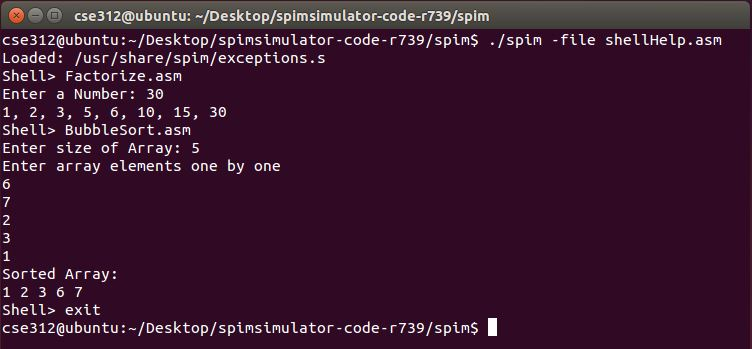
\includegraphics[width=6in, height=3in]{res.JPG}
	\caption[Optional caption]{}
	\label{}
\end{figure}                              

\end{document}